\setbeamercolor{background canvas}{bg=fitblue}
\begin{frame}
\frametitle{Teselace}
\begin{center}
\Huge {\color{white}Teselace}
\end{center}
\end{frame}
\setbeamercolor{background canvas}{bg=white}

\begin{frame}[fragile]
\frametitle{Teselace}
	\begin{itemize}
	\item Teselace je rozřezání jednoho primitiva na více spojených.
	\item Může se použít pro zjemnění geometrie
	\item Nachází se za vertex shaderem a před geometry shaderem.
	\item Složená ze 3 částí:
	\begin{itemize}
	\item Control Shader
	\item Generování primitiv/Teselace
	\item Evaluation Shader
	\end{itemize}
	\item Nový typ primitiva \textcolor{red}{GL\_PATCHES}
	\end{itemize}
  {\scriptsize
	\begin{minted}[frame=lines]{c++}
glPatchParameteri(GL_PATCH_VERTICES,10);//nastavi pocet vrcholu patche - 10
glDrawArrays(GL_PATCHES,0,100);//vykresli 10 patchu po 10 vrcholech
	\end{minted}
  }
	\begin{figure}[h]
	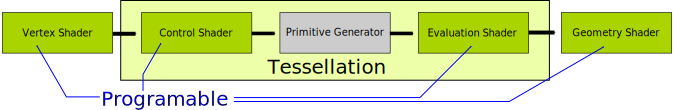
\includegraphics[width=10cm,keepaspectratio]{pics/tessellation/tess_pipeline.pdf}
	\end{figure}
\end{frame}

\begin{frame}
\frametitle{Control Shader}
	\begin{itemize}
	\item Řídí stupěň teselace
	\item Počítá kontrolní body
	\item Je spouštěn tolikrát, kolik je vertexů ve výstupním primitivu
	\item Číslo spuštění uloženo v \textcolor{OliveGreen}{gl\_InvocationID}
	\item \textcolor{OliveGreen}{barrier}()
	\end{itemize}
	\begin{figure}[h]
	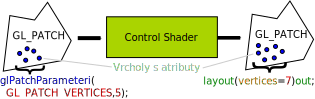
\includegraphics[width=10cm,keepaspectratio]{pics/tessellation/tess_control.pdf}
	\end{figure}
\end{frame}

\begin{frame}
    \frametitle{Parametry}

    
\includegraphics[width=\textwidth]{pics/tessellation/tess.pdf}

    \begin{itemize}
				\item \textcolor{OliveGreen}{layout}
					(\{\textcolor{orange}{isolines},\textcolor{orange}{triangles},\textcolor{orange}{quads}\})
					\textcolor{OliveGreen}{in};
				\item \textcolor{OliveGreen}{gl\_TessLevelOuter}[4],\textcolor{OliveGreen}{gl\_TessLevelInner}[2]
    \end{itemize}
\end{frame}

\begin{frame}[fragile]
\frametitle{Control Shader - příklad}
	{\scriptsize
	\begin{minted}[frame=lines]{glsl}
#version 430

// pocet vertexu ve vystupni primitivu
// pocet spusteni control shaderu
layout(vertices=3)out;

uniform vec2 TessLevelInner;//vnitrni deleni
uniform vec4 TessLevelOuter;//deleni hran

void main(){
  //velikost gl_in zavisi na GL_PATCH_VERTICES
  //velikost gl_out zavisi na layout(vertices=n)out;
  gl_out[gl_InvocationID].gl_Position=gl_in[gl_InvocationID].gl_Position;
  if(gl_InvocationID==0){
    gl_TessLevelOuter[0]=TessLevelOuter[0];
    gl_TessLevelOuter[1]=TessLevelOuter[1];
    gl_TessLevelOuter[2]=TessLevelOuter[2];
    gl_TessLevelOuter[3]=TessLevelOuter[3];
    gl_TessLevelInner[0]=TessLevelInner[0];
    gl_TessLevelInner[1]=TessLevelInner[1];
  }
}
	\end{minted}
	}
\end{frame}

\begin{frame}
\frametitle{Evaluation Shader}
	\begin{itemize}
		\item Nastavuje typ primitiva \textcolor{Orange}{isolines},\textcolor{orange}{triangles},\textcolor{orange}{quads}
		\item Počítá souřadnice vrcholů nateselovaného primitiva
		\item Souřadnice do primitiva \textcolor{OliveGreen}{gl\_TessCoord}
		\item je spoštěn pro každý nateselovaný vrchol
		\item vygenerovaná primitiva jdou dále do geometry shaderu
	\end{itemize}
	\begin{figure}[h]
	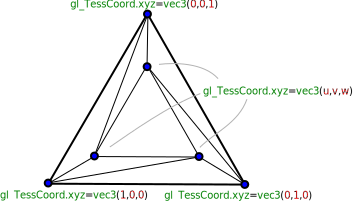
\includegraphics[width=7cm,keepaspectratio]{pics/tessellation/tess_coord.pdf}
	\end{figure}
\end{frame}


\begin{frame}[fragile]
\frametitle{Evaluation Shader - příklad}
	\begin{itemize}
		\item Nateselovaný čtyřúhelník
		\item výpočet pozic vrcholů
	\end{itemize}
	{\scriptsize
	\begin{minted}[frame=lines]{glsl}
#version 430

layout(quads)in;

void main(){
  vec4 A=mix(gl_in[0].gl_Position,gl_in[1].gl_Position,gl_TessCoord.x);
  vec4 B=mix(gl_in[3].gl_Position,gl_in[2].gl_Position,gl_TessCoord.x);
  gl_Position=mix(A,B,gl_TessCoord.y);
}
	\end{minted}
	}
\end{frame}




\begin{frame}[fragile]
  \frametitle{Béziérovy plochy - příklad}
	{\scriptsize
	\begin{minted}[frame=lines]{glsl}
// Vertex shader	
#version 430
void main() {
  gl_Position = mvp*position;
}

// Control shader
#version 430
layout(vertices=16) out;

void main() {
  gl_out[gl_InvocationID].gl_Position =
  gl_in[gl_InvocationID].gl_Position;
  if(gl_InvocationID == 0) {
    gl_TessLevelInner[0] = gl_TessLevelInner[1] = 
    gl_TessLevelOuter[0] = gl_TessLevelOuter[1] =
    gl_TessLevelOuter[2] = gl_TessLevelOuter[3] = 64;
  }
}
	\end{minted}
	}
\end{frame}

\begin{frame}[fragile]
    \frametitle{Béziérovy plochy - příklad}
  	{\scriptsize
		\begin{minted}[frame=lines]{glsl}
// Evaluation shader
#version 430
layout(quads, ccw) in;

vec4 bernstein(float t) {
  return vec4((1-t)*(1-t)*(1-t), 3*t*(1-t)*(1-t), 3*t*t*(1-t), t*t*t);
}

void main() {
  vec4 bu = bernstein(gl_TessCoord.x);
  vec4 bv = bernstein(gl_TessCoord.y);
  vec4 position = vec4(0, 0, 0, 0);
  for(int y = 0; y < 4; ++y){
    for(int x = 0; x < 4; ++x){
      position += bu[x]*bv[y]*gl_in[4*y + x].gl_Position;
    }
  }
  gl_Position = position;
}
  	\end{minted}
		}
\end{frame}

\begin{frame}[fragile]
\frametitle{Komunikace mezi shadery - příklad}
	{\tiny
	\begin{minted}[frame=lines]{glsl}
#version 430

//vertex shader
out vec4 vAttrib;
gl_Position

//control shader
//atribut z vertex shaderu jejich pocet je rizen glPatchParameteri(GL_PATCH_VERTICES,n);
in  vec4 vAttrib[];//atribut z vertex shaderu
gl_in[].gl_Position;//atribut pozice z vertex shaderu
//atribut z control shaderu do evaluation shaderu, pocet je rizen pomoci layout(vertices=n)out;
out vec4 cAttrib[];//atribut pro vrchol z control shaderu do evaluation shaderu
//per patch atribut z control shaderu do evaluation shaderu, pocet je 1
patch out mat4 cM;//atribut pro patch z control shaderu do evaluation shaderu

//evaluation shader
in vec4 cAttrib[];
patch in  mat4 cM;
//atribut z evaluation shaderu do geometry shaderu
out vec3 eNormal;

//geometry shader
//pocet je rizen typem primitiva
in vec3 eNormal[];
	\end{minted}
	}
\end{frame}

\begin{frame}[fragile]
    \frametitle{Příklad - Kružnice vepsaná}
  \begin{columns}[T]
    \begin{column}{.44\textwidth}
	    \begin{figure}[h]
    		\includegraphics[width=5cm,keepaspectratio]{pics/tessellation/ts_circle}
    	\end{figure}
    \end{column}
    \begin{column}{.48\textwidth}
 	    \begin{figure}[h]
    		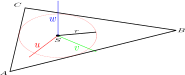
\includegraphics[width=5cm,keepaspectratio]{pics/tessellation/circle.pdf}
    	\end{figure}
{\tiny
$$
K=
\left( 
\begin{array}{cccc} 
1 & 0 & 0 & S_x \\
0 & 1 & 0 & S_y \\
0 & 0 & 1 & S_z \\
0 & 0 & 0 & 1  \\
\end{array}
\right)
\cdot
\left( 
\begin{array}{cccc} 
r & 0 & 0 & 0 \\
0 & r & 0 & 0 \\
0 & 0 & r & 0 \\
0 & 0 & 0 & 1  \\
\end{array}
\right)
\cdot$$
$$
\left( 
\begin{array}{cccc} 
u_x & v_x & w_x & 0 \\
u_y & v_y & w_y & 0 \\
u_z & v_z & w_z & 0 \\
0 & 0 & 0 & 1  \\
\end{array}
\right)
$$
}
    \end{column}
  \end{columns}
\end{frame}

\begin{frame}[fragile]
    \frametitle{Příklad - Kružnice vepsaná}
  \begin{columns}[T]
    \begin{column}{.44\textwidth}
      Control Shader
  	{\tiny
		\begin{minted}[frame=lines]{glsl}
#version 400
layout(vertices=1)out;
patch out mat4 K;
void main(){
  gl_TessLevelOuter[0]=1;
  gl_TessLevelOuter[1]=64;
  gl_TessLevelOuter[2]=1;
  gl_TessLevelOuter[3]=1;
  gl_TessLevelInner[0]=1;
  gl_TessLevelInner[1]=1;
  vec4 TT[3];
  TT[0]=gl_in[0].gl_Position;
  TT[1]=gl_in[1].gl_Position;
  TT[2]=gl_in[2].gl_Position;
  float t01=length((TT[0]-TT[1]).xyz);
  float t02=length((TT[0]-TT[2]).xyz);
  float t12=length((TT[1]-TT[2]).xyz);
  float s=t01+t02+t12;
  float r=sqrt((s/2-t01)*(s/2-t02)*(s/2-t12)*s/2)*2/s;
  t01/=s;
  t02/=s;
  t12/=s;
  vec3 C=TT[0].xyz*t12+TT[1].xyz*t02+TT[2].xyz*t01;
  vec3 x=normalize(TT[0].xyz-C);
  vec3 y=normalize(TT[1].xyz-C);
  vec3 z=normalize(cross(x,y));
  y=normalize(cross(z,x));
  K=mat4(vec4(x,0)*r,vec4(y,0)*r,vec4(z,0)*r,vec4(C,1));
}
  	\end{minted}
		}
    \end{column}
    \begin{column}{.48\textwidth}
      Evaluation Shader
  	{\tiny
		\begin{minted}[frame=lines]{glsl}
#version 400

#define MY_PI 3.14159265359

layout(isolines)in;

uniform mat4 V;
uniform mat4 P;

patch in mat4 K;

void main(){
  float Angle=gl_TessCoord.x*MY_PI*2;
  vec4 PP=vec4(cos(Angle),sin(Angle),0,1);
  gl_Position=P*V*K*PP;
}
  	\end{minted}
		}
    \end{column}
  \end{columns}

\end{frame}


\begin{frame}
\frametitle{Jak moc teselovat?}
	Outer level:
	\begin{itemize}
	\item Strany ploch musí odpovídat (zamezení T-spojů)
	\item Transformovat kontrolní body na obrazovku
	\item Spočítat delků hran
	\item Dělit maximální delkou hrany
	\end{itemize}
	Inner level:
	\begin{itemize}
	\item Z přílušných outer-levelů
	\item průměr, maximum, ...
	\item Korekce podle vnitřních kontrolních bodů
	\end{itemize}
	Ukázka v aplikaci
\end{frame}

